\UseRawInputEncoding
\begin{longtable}[c]{|c|c|c|c|}
\caption{Dimensi� dels fractals estudiats en aquest treball.}\\
\hline
\textbf{Valor real} & \textbf{Valor aproximat} & \textbf{Nom} & \textbf{Representaci�} \\
\hline
\endfirsthead
\multicolumn{4}{c}%
{\tablename\ \thetable\ -- \textit{Continua de la p�gina anterior}} \\
\hline
\textbf{Valor real} & \textbf{Valor aproximat} & \textbf{Nom} & \textbf{Representaci�} \\
\hline
\endhead
\hline \multicolumn{4}{r}{\textit{Continua en la p�gina seg�ent}} \\
\endfoot
\hline
\endlastfoot
\hline
$\frac{\log(2)}{\log(3)}$ & 0.6309 & conjunt de Cantor & \includegraphics[width=3.75cm, valign = c]{img/img02_03_cantor.pdf}\\
\hline
$\frac{\log(4)}{\log(3)}$ & 1.2619 & corba de Koch & \includegraphics[width=3.75cm, valign = c]{img/img02_04_koch.pdf}\\
\hline
$\frac{\log(3)}{\log(2)}$ & 1.585 & triangle de Sierpi\'{n}ski & \includegraphics[width=3.75cm, valign = c]{img/img02_05_sierpinski.pdf}\\
\hline
$\frac{\log(2)}{\log(3)}$ & 1.8928 & catifa de Sierpi\'{n}ski & \includegraphics[width=3.75cm, valign = c]{img/img02_06_carpet.pdf}\\
\hline
$\frac{\log(2)}{\log(\sqrt{2})}$ & 2 & corba de drac & \includegraphics[width=3.75cm, valign = c]{img/img03_dragon_curve.pdf}\\
\hline
$\frac{\log(4)}{\log(2)}$ & 2 & tetraedre de Sierpi\'{n}ski & \includegraphics[width=3.75cm, valign = c]{img/img02_08_tetraedro.pdf}\\
\hline
$\frac{\log(20)}{\log(3)}$ & 2,7268 & esponja de Menger & \includegraphics[width=3.75cm, valign = c]{img/img02_09_menger.pdf}\\
\hline
2 & 2 & corba de Peano & \includegraphics[width=3.75cm, valign = c]{img/img02_10_peano.pdf}\\
\hline
2 & 2 & conjunt de Julia & 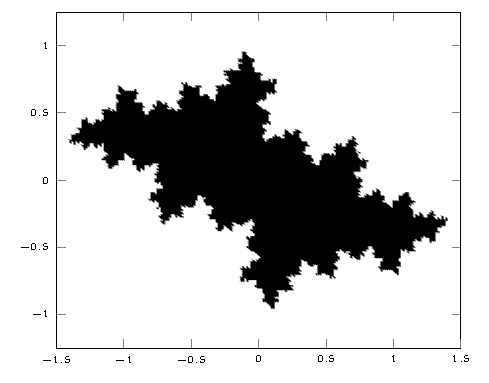
\includegraphics[width=3.75cm, valign = c]{img/img03_01_julia.pdf}\\
\hline
2 & 2 & conjunt de Mandelbrot & \includegraphics[width=3.75cm, valign = c]{img/img02_12_mandelbrot.pdf}\\
\hline
\end{longtable}
